% Section content template for individual Educative lessons
% This file contains the actual content for a specific section
% Generated from Educative API section content

% Section: Facebook, WhatsApp, Instagram, Oculus Outage
% Section ID: 5214324309622784
% Section Slug: facebook-whatsapp-instagram-oculus-outage
% Generated: 2025-12-08T15:37:16.908376

In October 2021, Facebook experienced a global outage for about six hours, affecting its other affiliates, including Messenger, WhatsApp, Mapillary, Instagram, and Oculus. Popular media reported the impact of this failure prominently. The
\emph{New York Times} reported the following headline: ``Gone in Minutes, Out for Hours: Outage Shakes Facebook.''
\\
According to one estimate, this outage cost Facebook about \$100 million in revenue losses and many billions due to the declining stock of the company.
\\
Let's look at the sequence of events that caused this global problem.

\subsection{The sequence of events}\label{WIIpVREk_OUtjlk2fMLAl}
\\
The following sequence of events led to the outage of Facebook and its accompanied services:

\begin{itemize}
\item
\protect\phantomsection\label{gCPiYptC3FFujZzIGoDVk}
A routine maintenance system was needed to find out the spare capacity on Facebook's backbone network.
\item
\protect\phantomsection\label{qSS_SyQzHsFxC7030FNDF}
Due to a configuration error, the maintenance system disconnected all the data centers from each other on the backbone network. Earlier , an automated configuration review tool was used to look for any issues in the configuration, but tools like these aren't perfect. In this specific case, the review tool missed the problems present in a configuration.
\item
\protect\phantomsection\label{PAJCx0SlMhjthzCenuWfB}
The authoritative domain name systems (DNSs) of Facebook had a health check rule that if it couldn't reach Facebook's internal data centers, it would stop replying to client DNS queries by withdrawing the routes.
\item
\protect\phantomsection\label{2rC9U17pLixcvWnpHc9-m}
When the networks routes where Facebook's authoritative DNS was hosted were withdrawn, all cached mapping of human-readable names to IPs soon timed out at all public DNS resolvers. When a client resolves \href{http://www.facebook.com}{www.facebook.com}, the DNS resolver first goes to one of the root DNS servers, which provides a list of authoritative DNS servers for \texttt{.com}. The resolver connects to one of them, and then they provide IPs for the authoritative DNS servers for Facebook. However, after route withdrawal, it was impossible to reach them.
\item
\protect\phantomsection\label{6JNdlFl1w6kUcvTo5Hthg}
Then, no one was able to reach Facebook and its subsidiaries.
\end{itemize}
\\
The slides below depict the events in pictorial form.

\begin{figure}[htbp]
 \centering
 \begin{subfigure}[b]{0.48\textwidth}
 \centering
 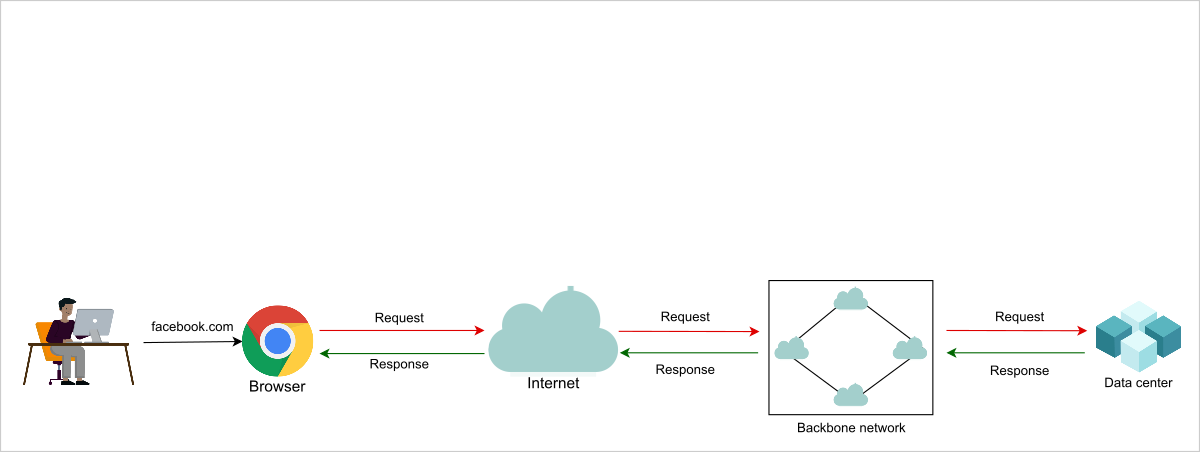
\includegraphics[width=\textwidth]{Images/chapter_42/section_5214324309622784/6578298079674368.png}
 \caption{Facebook’s high-level architecture}
 \end{subfigure}
 \hfill
 \begin{subfigure}[b]{0.48\textwidth}
 \centering
 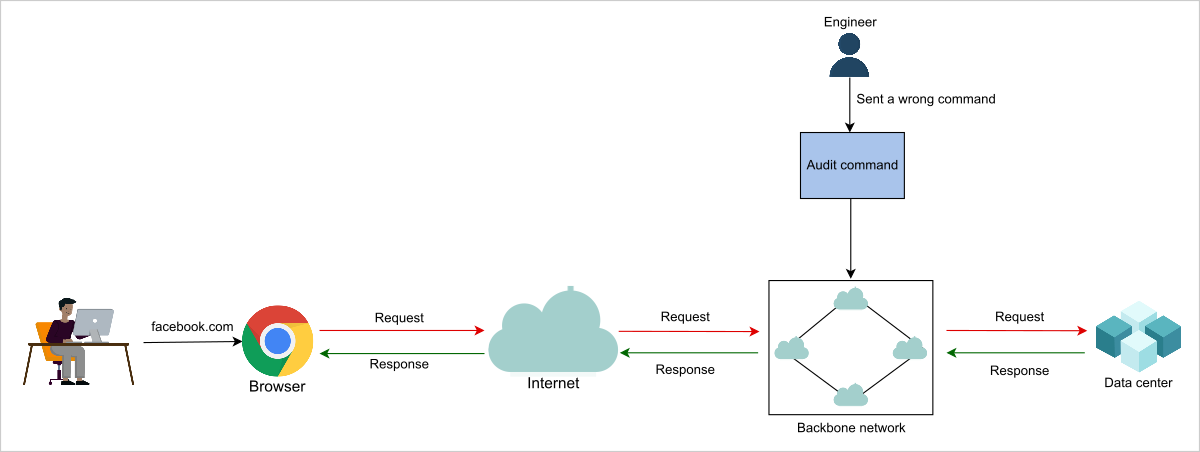
\includegraphics[width=\textwidth]{Images/chapter_42/section_5214324309622784/5518889152937984.png}
 \caption{A maintenance team sent the wrong commands to the backbone network}
 \end{subfigure}
\end{figure}

\begin{figure}[htbp]
 \centering
 \begin{subfigure}[b]{0.48\textwidth}
 \centering
 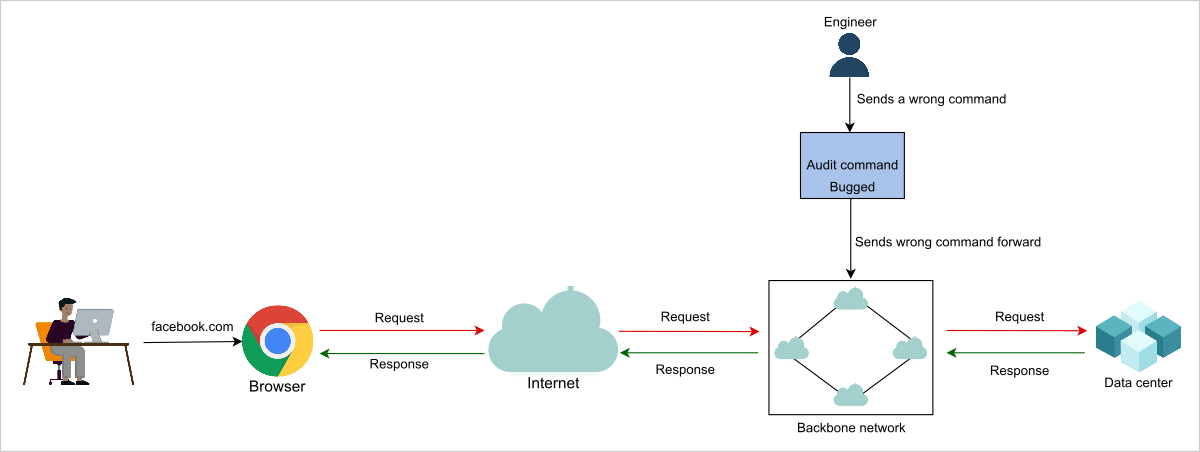
\includegraphics[width=\textwidth]{Images/chapter_42/section_5214324309622784/5854614880780288.png}
 \caption{The review tool (an audit command) couldn’t identify the problem with the command and sent the command forward to the backbone network}
 \end{subfigure}
 \hfill
 \begin{subfigure}[b]{0.48\textwidth}
 \centering
 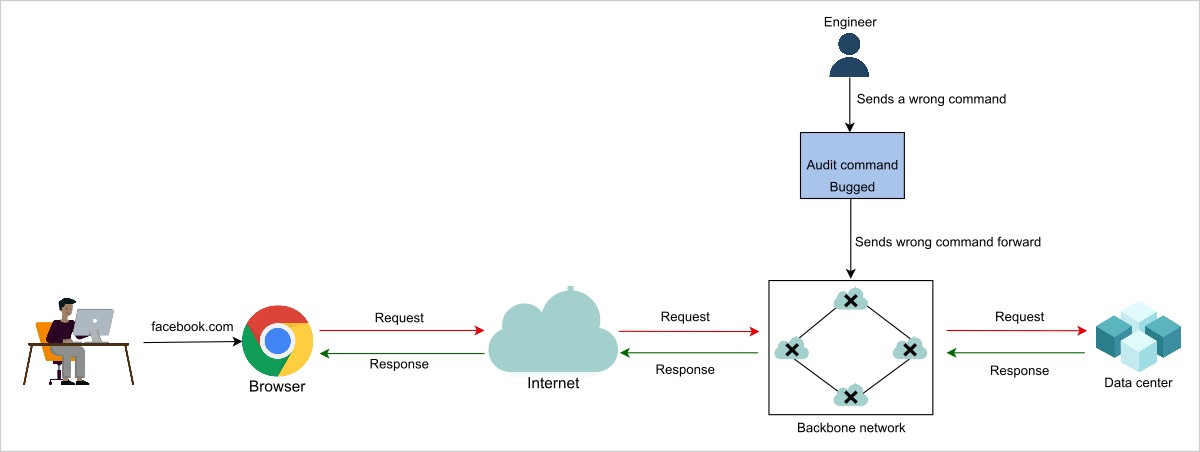
\includegraphics[width=\textwidth]{Images/chapter_42/section_5214324309622784/5215197988126720.png}
 \caption{Due to faulty commands, the backbone network malfunctioned}
 \end{subfigure}
\end{figure}

\begin{figure}[htbp]
 \centering
 \begin{subfigure}[b]{0.48\textwidth}
 \centering
 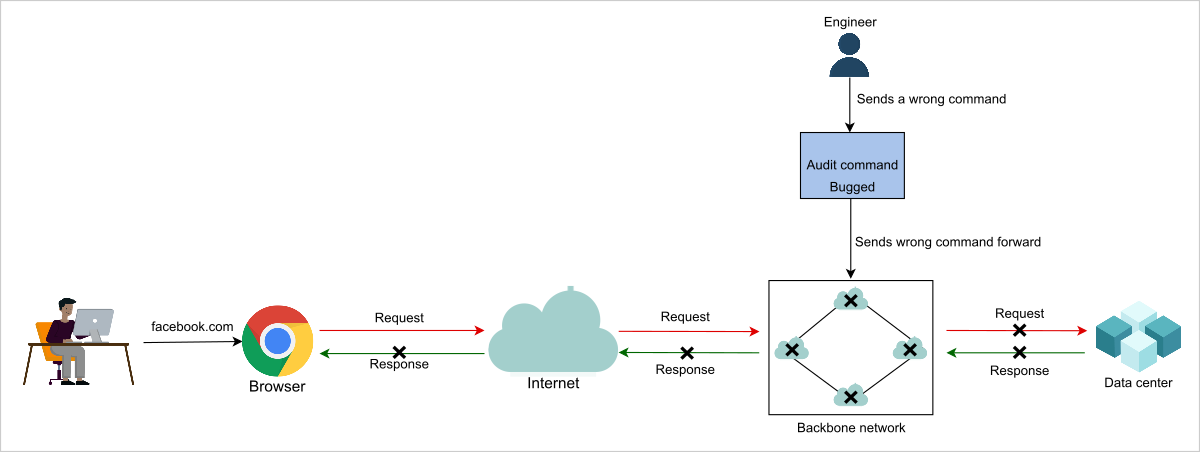
\includegraphics[width=\textwidth]{Images/chapter_42/section_5214324309622784/6480046005157888.png}
 \caption{As a result of the faulty commands, Facebook becomes unreachable}
 \end{subfigure}
\end{figure}

\subsection{Analysis}\label{6ld0oWBAMT8r5ulGkXUuU}
\\
Some of the key takeaways from the series of events shown above are the following:

\begin{itemize}
\item
\protect\phantomsection\label{Ska07B9X1Htxnvi5fmQXu}
\textbf{From common activity to catastrophe}: The withdrawal or addition of the network routes is a relatively common activity. The confluence of bugs (first a faulty configuration, and then a bug in an audit tool not able to detect such a problem) triggered a chain of events, which resulted in cascading failures. \textbf{A cascading failure} is when one failure can trigger another failure, ultimately bringing the whole system down.
\item
\protect\phantomsection\label{rPbjAdf05HNt9s0l77E0i}
\textbf{Reasons for slow restoration}: It might seem odd that it took six hours to restore the service. Wasn't it easy to reannounce the withdrawn routes? At the scale that Facebook is operating on, rarely is anything done manually, and there are automated systems to perform changes. The internal tools probably relied on the DNS infrastructure, and when all data centers are offline from the backbone, it would have been virtually impossible to use those tools. Manual intervention would have been necessary. Manually bootstrapping a system of this scale isn't easy. The usual physical and digital security mechanisms that were in place made it a slow process to intervene manually.
\item
\protect\phantomsection\label{TkCq7HmO1zYhYm77Yy_aE}
\textbf{Low probability events can occur}: In retrospect, it might seem odd that authoritative DNS systems disconnect themselves if internal data centers aren't accessible. This is another example where a very rare event, such as none of the data centers being accessible, happened, triggering another event.
\item
\protect\phantomsection\label{52CfpFSfydyBbnV2flOA_}
\textbf{Pitfalls of automation}: Facebook has been an early advocate of automating network configuration changes, effectively saying that software can do a better job of running the network than humans, who are more prone to errors. However, software can have bugs, such as this one.
\end{itemize}

\subsection{Lessons learned}\label{QdxxLP2lKeh1fPyYQmHKm}

\begin{itemize}
\item
\protect\phantomsection\label{N0Xbo3Zjw4AIm7UdBdOS-}
\textbf{Ready operations team}: There can be a hidden single point of failure in complex systems. The best defense against such faults is to have the operations team ready for such an occurrence through regular training. Thinking clearly under high-stress situations becomes necessary to deal with such events.
\item
\protect\phantomsection\label{a78AgaNaGzGfwglqNlAt0}
\textbf{Simple system design}: As systems get bigger, they become more complex, and they have emergent behaviors. To understand the overall behavior of the system, it might not be sufficient to understand only the behavior of its components. Cascading failures can arise. This is one reason to keep the system design as simple as possible for the current needs and evolve the design slowly. Unfortunately, there's no perfect solution to deal with this problem. We should accept the possibility of such failures, perform continuous monitoring, have the ability to solve issues when they arise, and learn from the failures to improve the system.
\item
\protect\phantomsection\label{-duQM95LuU2dSWLsVVnhm}
\textbf{Contingency plan}: Some third-party services rely on Facebook for single sign-on. When the outage occurred, third-party services were up and running, but their clients were unable to use them because Facebook's login facility was also unavailable. This is another example of assuming that some service will always remain available and of a hidden single point of failure.
\item
\protect\phantomsection\label{4_4WIAOf4d0pf9M9RZz50}
\textbf{Hosting DNS to independent third-party providers}: There are a few services that are so robustly designed and perfected over time that their clients start assuming that the service is and will always be 100\% available. The DNS is one such service, and it has been very carefully crafted. Designers often assume that it will never fail. Hosting DNS to independent third-party providers might be a way to guard against such problems. DNS allows multiple authoritative servers, and an organization might have many at different places. Although, we should note that DNS at Facebook's scale isn't simple, is tightly connected to their backbone infrastructure, and changes frequently. Delegating such a piece to an independent third party is expensive, and it might reveal internal service details. So, there can be a trade-off between business and robustness needs.
\item
\protect\phantomsection\label{ub-YjIjyq0ydWPaeRkjZW}
\textbf{Trade-offs}: There can be some surprising trade-offs. An example here is the need for data security and the need for rapid manual repair. Because so many physical and digital safeguards were in place, manual intervention was slow. This is a catch-22 situation---lowering security needs can cause immense trouble, and slow repair for such events can also make it hard for the companies. The hope is that the need for such repairs is a very rare event.
\item
\protect\phantomsection\label{EJfwDo9Chc1usslbGQ5hy}
\textbf{Surge in load}: The failure of large players disrupts the entire Internet. Third-party public resolvers, such as Google and Cloudflare, saw a surge in the load due to unsuccessful DNS retries.
\item
\protect\phantomsection\label{dqu0CKjvMujCbjNCwXUCu}
\textbf{Resuming the service}: Restarting a large service isn't as simple as flipping a switch. When the load suddenly becomes almost zero, turning them up suddenly may lead to a many megawatt uptick in power usage. This might even cause issues for the electric grid. Complex systems usually have a steady state, and if they go out of that steady state, care must be taken to bring them back.
\end{itemize}

\begin{quote}
\textbf{Quiz:}
\textbf{Question 1:} What can we do to safeguard against the kinds of faults experienced by

Facebook?
\textbf{Answer:} Some possible solutions can look like the following: * \#key\# Network verification: Network verification is the usage of network tools to investigate, troubleshoot, maintain, operate, and report to ensure that hardware, software, and network configuration will operate error-free.

\#key\# has recently gained momentum and has shown promise in catching bugs early on. Such tools use an abstract model of the infrastructure. *

There can be more than one layer of auditing. Second layers might use a simulator to make sure that after the configuration changes, critical network infrastructures remain available from multiple global vantage points. * Every effort should be taken to reduce the scope of a configuration change to avoid cascading effects. * Critical infrastructure might be programmed in such a way that if something bad happens, it could return to the last known good state. This is easier said than done owing to the sheer number of components.
\end{quote}



% End of section content